\subsection{Case study \#1: Debugging microbursts}
\label{s:eval:mininet}
\label{sec:eval:mininet}

To demonstrate \TheSystem in practice, we present a case study of
diagnosing microbursts, \ie spikes in latency caused by bursty
transmissions of packets into a queue.
%with a topology shown in Figure~\ref{fig:mininet-topo}.
Our setup in Mininet~\cite{mininet} consists of four hosts
({\ct h1, h2, h3, h4}) and two switches ({\ct S1, S2}) in a dumbbell topology.
Switch {\ct S1} is connected to {\ct h1} and {\ct h3},
and {\ct S2} to {\ct h2} and {\ct h4}.
The switches are connected via a single link and
programmed in P4~\cite{p4-bmv2} with queries compiled by \TheSystem.

Host {\ct h2} repeatedly downloads a 1MB objects over TCP from {\ct h1}.
Meanwhile, {\ct h3} sends {\ct h4} bursts of UDP traffic, which
{\ct h4} acks.  Suppose a network operator notices the irregular latency
spikes for the downloads (\Fig{mininet-latency}). She suspects a queue buildup
in the switches and measures the queue depths seen by the traffic by writing:
{\ct result = filter(\pktlog, srcip == h1 and dstip == h2).}

% Can remove this figure if we need space.
%\begin{figure}[ht]
%\centering
%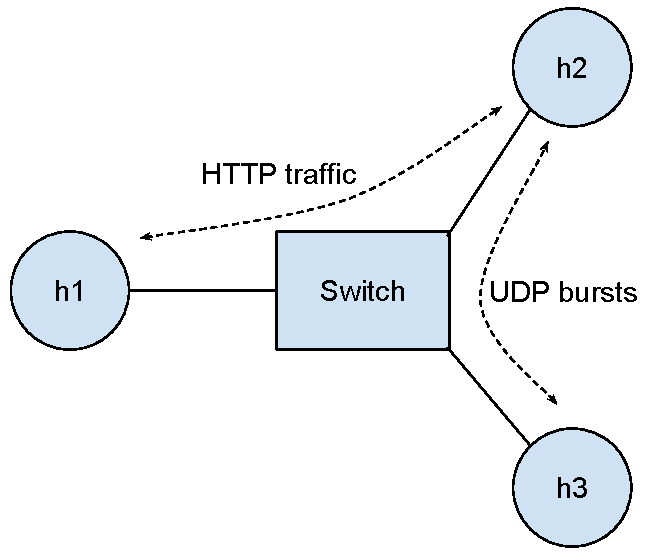
\includegraphics[width=0.4\columnwidth]{mininet-topo.pdf}
%\caption{Mininet topology used for the case study.}
%\label{fig:mininet-topo}
%\end{figure}

\begin{figure}[!t]
\centering
\begin{subfigure}[t]{0.48\columnwidth}
\raggedright
\includegraphics[width=\linewidth]{fetch_latency.pdf}
\vspace{-0.2in}
\caption{TCP request latency}
\label{fig:mininet-latency}
\end{subfigure}
\begin{subfigure}[t]{0.48\columnwidth}
\raggedleft
\includegraphics[width=\linewidth]{queue_sizes.pdf}
\vspace{-0.2in}
\caption{Queue depth at egress port 2}
\label{fig:mininet-qin}
\end{subfigure}
\vspace{-0.1in}
\caption{Microburst case study measurements.}
\end{figure}
\begin{figure}[t]
\vspace{0.083in}
\centering
\small
\begin{tabular}{c c c c c} \hline
\textbf{src $\rightarrow$ dst} & \textbf{protocol} & \textbf{\# Bursts} & \textbf{Time ($\mu$s)} & \textbf{\# Packets} \\ \hline \hline
h3:34573 $\rightarrow$ h4:4888 & UDP & 19 & 8969085 & 6090  \\ \hline
h4:4888 $\rightarrow$ h3:34573 & UDP & 18 & 10558176 & 5820 \\ \hline
h1:1777 $\rightarrow$ h2:58439 & TCP & 1 & 72196926 & 61584 \\ \hline
h2:58439 $\rightarrow$ h1:1777 & TCP & 1 & 72248749 & 33074 \\ \hline
\end{tabular}
\vspace{-0.1in}
\caption{Per-flow burst statistics from \TheSystem.}
\label{fig:mininet-flowstats}
\vspace{-0.1in}
\end{figure}

The results are streamed out on each packet to a collection server. After
plotting the queue latencies, she notices spikes in queue size at egress port 3
on the switch (\Fig{mininet-qin}) matching the periodicity of the latency
spikes. To isolate the responsible flow(s), she divides the traffic into
``bursts,'' which she defines as a series of packets separated by a gap of at
least 800ms, as determined from the gap between latency spikes. She issues the
following \TheSystem query:

\begin{small}
\begin{lstlisting}
def burst_stats([last_time, nburst, time], [pkts, tin]):
    if tin - last_time > 800000:
        nbursts++;
        emit();
    else:
        time = time + tin - last_time;
    pkts = pkts + 1;
    last_time = tin;
result = groupby(R1, (*\codeftuple{}*), burst_stats)
\end{lstlisting}
\end{small}

%%\vspace{-0.1in}
She runs the query for 72 seconds and sees the result in
\Fig{mininet-flowstats}. She concludes, correctly, that UDP traffic between
{\ct h3} and {\ct h4} is responsible for the latency spikes.  There are 18 UDP
bursts, with an average packet size and duration
%of 320 packets and average duration of 472 ms,
that matches our emulation setup.

\TheSystem's flexibility makes this diagnosis simple.
%
By contrast, localizing the root cause of microbursts with existing monitoring
approaches is challenging.
%
Packet sampling and
line-rate packet captures would miss microbursts because of heavy undersampling,
packet counters from switches would have disguised the bursty nature of the
offending UDP traffic, and probing from endpoints would not be able to
localize queues with bursty contending flows.

\TheSystem builds on In-band Network Telemetry~\cite{int, barefoot-demo} (INT)
that exposes queue lengths at switches. However, \TheSystem's on-switch
aggregation goes beyond INT to determine contending flows at the problematic
queue through a customized query, without prior knowledge of those flows.
%
In comparison, a pure INT-based solution may require a network operator to
manually identify flows that could contend at the problematic queue, and then collect data
from the INT endpoints for those flows.
